% Author: Zhehao Wang 404380075 zhehao@cs.ucla.edu

% Grammar package: http://tex.stackexchange.com/questions/24886/which-package-can-be-used-to-write-bnf-grammars

\documentclass{article}
\topmargin = 0in
\oddsidemargin = 0in
\evensidemargin = \oddsidemargin
\textwidth = 6.5in
\textheight = 8in
\usepackage{amsthm}
\usepackage{amsmath}
\usepackage{syntax}
\usepackage{graphicx}

\usepackage{algorithm}
\usepackage[noend]{algpseudocode}

\makeatletter
\def\BState{\State\hskip-\ALG@thistlm}
\makeatother

\title{CS180 Homework 3}
\author{Zhehao Wang 404380075 (Dis 1B)}
\date{Apr 16, 2016}

\begin{document}
\maketitle

\begin{description}

\item[1]{Strongly connected components in a directed graph}
  
  (a) Prove SCC graph is a DAG.

  \textbf{Proof by contradiction:} assume that a path $s_i, ..., s_j, s_i$ exists in the SCC graph, where $s_k$ ($i \leq k \leq j$) are the newly created distinct SCC nodes.

  Consider a node $p_i$ in SCC node $s_i$, there exists a path from $p_i$ to any node $p_{i+1}$ in SCC $s_{i+1}$, since there exists a node $q_i$ in SCC $s_i$ that has a directed edge to a node $q_{i+i}$ in SCC $s_{i+1}$, and there exists a path from $p_i$ to $q_i$ and from $q_{i+1}$ to $p_{i+1}$.

  Starting from $p_i$, apply the above conclusion repeatedly till we reach a node $p_j$ in SCC $s_j$, and we have that there exists a path from $p_i$ to $p_j$. Similarly, we have there exists a path from $p_j$ to $p_i$. Thus the nodes $p_i$ and $p_j$ should belong to the same SCC node which is the combination of SCC nodes $s_i$ and $s_j$. This contradicts with the nodes being distinct in the assumption. Thus we have the directed SCC graph is acyclic, which makes it a DAG by definition.

  (b) The algorithm is given in alg \ref{alg:scc-graph}. 

  This algorithm does not follow the hint to the word (which we suspect to be misleading, as explained in the \textbf{notes} section below). Instead, the \textit{reverse} post order labeling using DFS and the subsequent DFS traversals starting from the smallest label (we start from smallest as the algorithm does a \textit{reverse} post order labeling) are done in one pass. 

  To reduce complexity, the algorithm involves bookkeeping which labels all the nodes according to the sequences they are visited (This $index$ does not reflect the sequence of subsequent DFS traversals, which follows the reverse post order of the graph), and uses $lowlink$ to keep track of the label of the SCC the node's in, which is the smallest index of all nodes in the SCC.

  The algorithm is invoked by calling $tarjanSCC(G)$, and should output (line \ref{line:output}) the list of nodes in each SCC.

  \begin{algorithm}[H]
  \caption{SCC building algorithm (Tarjan)}
  \label{alg:scc-graph}
    \begin{algorithmic}[1]
    \Function{tarjanSCC}{G}
      \State $index \gets 0$
      \State $stack \gets []$
      \For {$\{v \in V\}$}
        \If {$v.index = nil$}
          \State $scc(v)$
        \EndIf
      \EndFor

      \Function{scc}{v}
        \State $v.index \gets index$
        \State $v.lowlink \gets index$
        \State $index \gets index + 1$
        \State $SCC\_nodes \gets []$

        \State $stack.push(v)$
        \State $v.onStack \gets true$

        \For {$\{w | (v,w) \in E\}$}
          \If {$w.index = nil$}
            \State $scc(w)$
            \State $v.lowlink \gets min(v.lowlink, w.lowlink)$
          \ElsIf {$w.onStack$}
            \State $v.lowlink \gets min(v.lowlink, w.index)$
          \EndIf
        \EndFor

        \If {$v.lowlink = v.index$}
          \While {$w \neq v$}
            \State $w \gets stack.pop()$
            \State $w.onStack \gets false$
            \State $SCC\_nodes.addCurrent(w)$
          \EndWhile
        \EndIf
        \State $SCC\_nodes.output()$
        \label{line:output}
      \EndFunction

    \EndFunction

    \end{algorithmic}
  \end{algorithm}

  \textbf{Time complexity:} this algorithm is $O(|E|)$. The initial labeling DFS traversal visits each edge exactly once and is $O(|E|)$. All the subsequent DFSs combined also visits each edge exactly once, and is $O(|E|)$. So the overall complexity is $O(|E|)$.

  \textbf{Correctness:} Let $G=(V,E)$ be the original graph, according to the algorithm description, we want to first prove that for all $r \in V$, by the time DFS finishes $r$, let the tree built by the DFS be $G'=(V',E')$, if there exists a path $p_i$ in $E$ that starts from $r$ to any $n \in V'$, then $n$ and $r$ belongs to the same SCC. Then we can merge these two nodes, continue with the DFS recursively, and use the same criteria to tell which SCC the next finished node belongs to, until all nodes are finished. 

  Consider the case when DFS finishes the first node $r$, $E'$ would contain only one path from the starting point of DFS $v$ to the sink $r$. Thus any node $v' \in V'$ has a path to $r$. Given that there exists a path from $r$ to any $n \in V'$ and there exists a path from $n$ to $r$, $r$ and $n$ should be in the same SCC, and the first part of the conclusion holds. After merging $n$ and $r$, we face a subproblem of the original problem with 1 less node, which we can solve by continuing with the recursion. 

  \textbf{Note:} following the hint to the word may not result in a correct algorithm. Consider the graph in \ref{fig:pb1}, with a DFS starting from $a$, if the DFS chooses the rightmost path first, we have a post order traversal order of $a, b, d, e, c$; according to the hint, we then start from $c$, do a DFS, which will lead us to think that $c, b, d, e$ are in an SCC, which is not the case here. 

  The difference between the hint and Tarjan's algorithm as given above, seems to be that Tarjan's algorithm essentially does the first labeling DFS run and subsequent DFS runs in one pass (in this example, the nodes $c, b$ will be taken out as a SCC before $d$ is explored.)

  \begin{figure}[h]
  \centering
  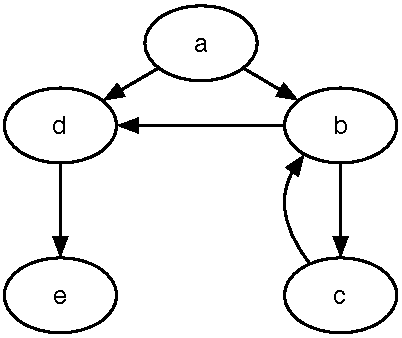
\includegraphics[width=0.25\textwidth]{hw31case}
  \caption{Problematic case with just following the hint}
  \label{fig:pb1}
  \end{figure}

\item[2]{Longest path in DAG}

  (a) algorithm is given in alg \ref{alg:longest-path-unweighted-dag}. As we find new sources, we update the \textit{from} field of the node to keep track of the nodes on the longest path.

  \begin{algorithm}[h]
  \caption{Longest path in an unweighted DAG}
  \label{alg:longest-path-unweighted-dag}
    \begin{algorithmic}[1]
  
    \Function{longestPath}{G}
      \State $nodeCount \gets len(V)$
      \State $sourceNodes \gets []$
      \State $lastNode \gets nil$
      \For {$\{i|i \in V\}$}
        \If {$i.inDegree = 0$}
          \State $sourceNodes.add(i)$
        \EndIf
      \EndFor
      \State $length \gets 0$
      \While {$nodeCount > 0$}
        \State $newSourceNodes \gets []$
        \For {$\{i|i \in sourceNodes\}$}
          \For {$\{v|(i, v) \in E\}$}
            \State $v.inDegree \gets v.inDegree - 1$
            \If {$v.inDegree = 0$}
              \State $newSourceNodes.add(v)$
              \State $v.from \gets i$
            \EndIf
          \EndFor
          \State $G.remove(i)$
          \State $lastNode \gets i$
          \State $nodeCount \gets nodeCount - 1$
        \EndFor
        \State $sourceNodes \gets newSourceNodes$
        \State $length \gets length + 1$
      \EndWhile

      \State $node \gets lastNode$
      \State $path \gets [lastNode]$
      \While {$node.from \neq nil$}
        \State $path.push(node.from)$
        \State $node = node.from$
      \EndWhile
      \State \Return $length$, $path$
    \EndFunction
    
    \end{algorithmic}
  \end{algorithm}

  \textbf{Time complexity:} this iterative algorithm is $O(|E|)$, as it's using an $O(|E|)$ topological sorting algorithm with number of phases remembered. 

  \textbf{Correctness:} this algorithm counts the phases needed to remove all nodes in a topological sort. The correctness is based on the conclusion that length of longest path in a DAG $G$ is 1 + length of longest path in $G'$, where $G'$ is the remaining graph after all sources in $G$ are removed. This conclusion can be proved by induction.

  Base case obviously holds for graphs with only one node, or two nodes with one directed edge between them.

  Induction hypothesis: conclusion holds for any DAGs that takes $n$ phases in a topological sort, and the longest path is $n-1$.

  Induction case holds for graphs that take $n+1$ phases. Proof by contradiction: assume there's a longer path than $n$ (at least $n+1$), the sub graph with all sources removed need to have length at least $n$, which contradicts with the induction hypothesis.

  (b) algorithm is given in alg \ref{alg:longest-path-weighted-dag}. Similar with (a), we label each node. Each time the algorithm removes a source node $i$, the nodes $j$ that it connects to will have the label $w(j) = max(w(j), l(i,j) + w(i))$. The largest label in the DAG will be the length of the longest path. As we update the label with larger values, we update the \textit{from} field of the node to keep track of the longest nodes on the path.

  \begin{algorithm}[h]
  \caption{Longest path in a weighted DAG}
  \label{alg:longest-path-weighted-dag}
    \begin{algorithmic}[1]
  
    \Function{longestPath}{G}
      \State $nodeCount \gets len(V)$
      \State $sourceNodes \gets []$
      \State $maxNode \gets nil$
      \For {$\{i|i \in V\}$}
        \If {$i.inDegree = 0$}
          \State $sourceNodes.add(i)$
          \State $i.label \gets 0$
        \EndIf
      \EndFor
      \State $maxLength \gets 0$
      \While {$nodeCount > 0$}
        \State $newSourceNodes \gets []$
        \For {$\{i|i \in sourceNodes\}$}
          \For {$\{v|(i, v) \in E\}$}
            \State $v.inDegree \gets v.inDegree - 1$
            \If {$v.label < i.label + l(i,v)$}
              \State $v.label \gets i.label + l(i,v)$
              \State $v.from \gets i$
            \EndIf
            \If {$maxLength < v.label$}
              \State {$maxLength \gets v.label$}
              \State {$maxNode \gets v$}
            \EndIf
            \If {$v.inDegree = 0$}
              \State $newSourceNodes.add(v)$
            \EndIf
          \EndFor
          \State $G.remove(i)$
          \State $nodeCount \gets nodeCount - 1$
        \EndFor
        \State $sourceNodes \gets newSourceNodes$
      \EndWhile

      \State $node \gets maxNode$
      \State $path \gets [maxNode]$
      \While {$node.from \neq nil$}
        \State $path.push(node.from)$
        \State $node = node.from$
      \EndWhile
      \State \Return $maxLength$, $path$
    \EndFunction
    
    \end{algorithmic}
  \end{algorithm}

  \textbf{Time complexity:} similar with a topological sort, this algorithm is $O(|E|)$, as each edge in the graph will be used exactly once.

  \textbf{Correctness:} 

  \textbf{Lemma:} during the topological sort, every time a node $p$ becomes source, its label will be the length of the longest path starting from any node and ending at $p$. 

  This lemma is easily proved by contradiction, as when the node becomes source there won't be any path going to it, so the label of the source will be the length of maximum path that ends at the node. (The labels of all nodes are initialized as 0, so that negative labels won't be kept, and in case of negative labels, we could just ignore the earlier paths that lead to this node.)

  The algorithm returns the maximum label of nodes in the graph after all nodes become sources, given the lemma, the algorithm will return the length of the longest path in the graph.

  (c) algorithm is given in alg \ref{alg:weighted-dag-job-scheduling}. Similar as (b), the algorithm labels jobs, and returns a list of jobs sorted by their labels (defined as the longest time it takes to get the prerequisites of that job done). A schedule that starts each job at the labeled time minimizes the total time needed to finish all jobs.

  \begin{algorithm}[h]
  \caption{Weighted DAG job scheduling}
  \label{alg:weighted-dag-job-scheduling}
    \begin{algorithmic}[1]
  
    \Function{longestPath}{G}
      \State $nodeCount \gets len(V)$
      \State $sourceNodes \gets []$
      \For {$\{i|i \in V\}$}
        \If {$i.inDegree = 0$}
          \State $sourceNodes.add(i)$
          \State $i.label \gets 0$
        \EndIf
      \EndFor
      \While {$nodeCount > 0$}
        \State $newSourceNodes \gets []$
        \For {$\{i|i \in sourceNodes\}$}
          \For {$\{v|(i, v) \in E\}$}
            \State $v.inDegree \gets v.inDegree - 1$
            \State $v.label \gets max(v.label, i.label + l(i))$
            
            \If {$v.inDegree = 0$}
              \State $newSourceNodes.add(v)$
            \EndIf
          \EndFor
          \State $G.remove(i)$
          \State $nodeCount \gets nodeCount - 1$
        \EndFor
        \State $sourceNodes \gets newSourceNodes$
      \EndWhile
      \State \Return $sort(v.label)$
    \EndFunction
    
    \end{algorithmic}
  \end{algorithm}

  \textbf{Time complexity:} this algorithm is $O(max(|E|, |V| \log |V|))$. $O(|E|)$ comes from the topological sort and labeling, which will visit each edge exactly once; and $|V| \log |V|$ comes from the sorting by label in the end.

  \textbf{Correctness:} the proof is similar as that of (b) except that we don't need to consider the negative label case. A brief description below:

  \textbf{Lemma:} during the topological sort, when a node becomes source, its label is the earliest time when the corresponding job can start. This can be easily proved by induction given the label definition in alg \ref{alg:weighted-dag-job-scheduling}.

  By the lemma, we have that the algorithm provides a schedule that starts a job as soon as it can be started. This schedule is optimal, which can be easily proved by contradiction.

\item[3]{Optimal order of files}
  
  Algorithm is given in alg \ref{alg:optimal-order-of-files}, which is a greedy algorithm that orders files as $f_{t_1}...f_{t_n}$, such that for each $t_i > t_j$, $\frac{p_{t_i}}{l_{t_i}} \geq \frac{p_{t_j}}{l_{t_j}}$.

  \begin{algorithm}[h]
  \caption{Optimal order of files}
  \label{alg:optimal-order-of-files}
    \begin{algorithmic}[1]
  
    \Function{optimalOrder}{files}
      \State $weightedFiles \gets []$
      \For {$\{i|i \in files\}$}
        \State $weightedFiles.add(\frac{p_i}{l_i})$
      \EndFor
      \State \Return $sort(weightedFiles)$
    \EndFunction
    
    \end{algorithmic}
  \end{algorithm}

  \textbf{Time complexity:} this algorithm is $O(n \log n)$, where $n$ is the number of files. The calculation of $\frac{p_i}{l_i}$ requires a traversal of array, which is $O(n)$, and the sorting afterwards is $O(n \log n)$, which makes the entire algorithm $O(n \log n)$.

  \textbf{Correctness:} proof by the algorithm's greedy choice property and optimal substructure property.

  \textbf{Greedy choice property:} there exists an optimal solution $S=f_{t_1}...f_{t_n}$, such that $\frac{p_{t_1}}{l_{t_1}}$ is the largest among all jobs.

  % The assumed optimal solution takes a specific form, is this Ok in the proof; if not, is Ang's proof for maximum contatenation correct in dis 3? The idea of that one is bubble sorting, should be better described in the notes as well
  Proof: suppose $S'$ is an optimal solution with the sequence $f_{t'_1}f_{t'_2}...f_{t_{k-1}}f_{t_1}f_{t_{k+1}}...f_{t_n}$ where $t'_1 \neq t_1$. The average access time of $S'$ is 

  $$t(S') = \sum_{i=2}^{n}{((\sum_{j=1}^{i-1}{l_{t'_j}}) \cdot p_{t'_i})}$$

  Consider the solution $S''$ with $f_{t_1}$ and $f_{t_{k-1}}$ swapped, the difference between average access time of $S''$ and that of $S'$ is

  $$t(S') - t(S'') = p_{t_{1}} * l_{t_{k-1}} - p_{t_{k-1}} * l_{t_1} = (\frac{p_{t_1}}{l_{t_1}} - \frac{p_{t_{k-1}}}{l_{t_{k-1}}}) \cdot l_{t_1} \cdot l_{t_{k-1}} \geq 0$$

  Similarly, starting from $t(S'')$, each time we swap $f_{t_1}$ with its previous file, we'll have a smaller or equal access time than before. Thus the optimal solution should contain $f_{t_1}$ as its first element, whose $\frac{p_{t_1}}{l_{t_1}}$ is the largest.

  \textbf{Optimal substructure property:} let $S=f_{t_1}...f_{t_n}$ be an optimal solution, then $S_1=f_{t_2}...f_{t_n}$ is the optimal solution for the sub problem without $f_{t_1}$.

  Proof by contradiction: assume there's a better solution $S'_1=f_{t''_2}...f_{t''_n}$, $t(S'_1)<t(S_1)$ for the sub problem without $f_{t_1}$. Then $S'=f_{t_1}S'_1$ has the average access time of $t(S')=t(S'_1) + l_{t_1} * (1-p_{t_1}) < t(S_1) + l_{t_1} * (1-p_{t_1}) = t(S)$, which contradicts with $S$ being the optimal solution for the original problem.

  With both properties, the greedy algorithm in question is correct.

\item[4]{Sorting from SC}
  
  Suppose that $SC(p_i, d_i)$ takes in $n$ jobs, and each has a $p_i$ and $d_i$. $SC$ returns the optimal list of jobs expressed in two arrays $times$, $deadlines$. The sorting algorithm is described in alg \ref{alg:sorting-sc}.

  \begin{algorithm}[h]
  \caption{Sorting using SC}
  \label{alg:sorting-sc}
    \begin{algorithmic}[1]
  
    \Function{sort}{array}
      \State $times, deadlines \gets SC(array, array)$
      \State \Return $deadlines$
    \EndFunction
    
    \end{algorithmic}
  \end{algorithm}

  \textbf{Time complexity:} SC is $o(n \log n)$, and other calls are $O(1)$, so the overall $sort$ is $o(n \log n)$.

  \textbf{Correctness:} suppose that the algorithm gives back a deadline array of $S=d_1...d_n$, we want to prove for each $i<j$, $d_i \leq d_j$.

  We start by proving that the first element $d_1$ is a smallest element. 

  Assume we have a smaller element $d_k < d_1$ in $S$, $1 \leq i \leq n$. Let the maximum lateness of $S$ be $t(S) = max((\sigma_{i=1}^{n}{p_i}) - d_n)$. Consider the sequence $S'$ with $d_k$ and $d_{k-1}$ swapped, let its maximum lateness be $t(S')$. With given input where $p_i = d_i$, $t(S) = \sigma_{i=1}^{k-1}{d_i}$, $t(S') = \sigma_{i=1}^{k-2}{d_i} + d_k$, and $t(S) - t(S') = d_{k-1} - d_k \geq 0$. \footnote{With $SC$ being a blackbox, this given input only seems to guarantee the last element in the returned array has the largest deadline, and does not have other properties. A better solution would be to carefully craft a $p_i$ array to give to the input. An ideal $p_i$ array would be $p_i$ = $d_{i+1} - d_i$, where $d_i$ array is sorted, however this array can only be known after we have the sorting result...}

  Similarly, starting from $S'$, we repeatedly switch $d_k$ with its previous element, and can prove $t(S) \geq...\geq t(S_{k-1}) \geq t(S_k)$. Thus for $SC$ to provide the optimal solution, the first element $d_1$ should be a smallest element.

  Consider the array $S_1$ which is $S$ with $d_1$ removed, using the above described process we can prove that $d_2$ is a smallest element in $S_1$. We continue until the array $S$ is exhausted, and we have for each $i<j$, $d_i \leq d_j$.

\end{description}

\end{document}
